%%%%%%%%%%%%%%%%% your_thesis_eng.tex %%%%%%%%%%%%%%%%%
%
% This is the template file for ORM 2016 proceedings.
%
% Please, fill in following the directions below.
%
%%%%%%%%%%%%%%%%%%%%%%%%%%%%%%%%%%%%%%%%%%%%%%%%%%%%%%%

\newcommand{\No}{No.}

\Title[%
% Insert here the acknowledgements of grants and/or any other information you
% wish to appear as a footnote, or leave this field blank.
The reported study was funded by RFBR according to the research project \No
16-01-00353a.%
] {%
  % Insert your title here
  Multistage Bidding Model with Elements of Bargaining. Extension for a
  Countable State Space%
} {%
  % Insert the authors' names here
  A.I.~Pyanykh%
} {%
  % Insert your institution here
  Moscow State University%
} {%
  % Insert your city here
  Moscow%
} {%
  % Insert your country here
  Russia%
}

% Insert your thesis here. The entire submission should not exceed 3 pages if
% you plan a publication in conference proceedings.
%
% ATTENTION: Using 'thebibliography' environment is not allowed. Use
% 'references_eng' environment below to format the list of references. Please
% note that the latter environment does not provide automatic citation
% facilities. Cite manually using square brackets, e.g., [1], [2, 3], [4--6].
%
We consider a simplified model of a financial market with two players bidding
for one unit of a risky asset for $n \leq \infty$ consecutive stages. Player 1
(an insider) is informed about the liquidation price $s^0$ of the asset while
Player 2 knows only its probability distribution $p$. At each stage players
place integral bids. The higher bid wins, and an asset is transacted to the
winning player. Each player aims to maximize the value of her final portfolio.

A model where the price $s^0$ has only two possible values $\{0, m\}$ is
considered in [1]. It is reduced to a zero-sum game $G_n(p)$ with incomplete
information on one side as in Aumann, Maschler [2]. In this model uninformed
Player 2 uses the history of Player 1's moves to update posterior probabilities
over the liquidation price. Thus, Player 1 should find a strategy controlling
posterior probabilities in such a way that allows her to use the private
information without revealing too much of it to Player 2. The main results in
[1] are explicit optimal strategies and the value of the infinitely long game
$G_\infty(p)$. In [3] the model is extended so that the liquidation price can
take any value $s \in S = \mathbb{Z}_+$ according to a probability distribution
$p = (p_s, s \in S)$. It is shown that when $\mathbb{D}p$ is finite a game
$G_\infty(p)$ is properly defined. For this game the value and optimal players
strategies are found.

In both [1] and [3] the transaction price equals to the highest bid. Instead we
could consider a transaction rule proposed in [4], and define a transaction
price equal to a convex combination of proposed bids with a coefficient $\beta
\in [0, 1]$. A model with such transaction rule and two possible values of the
liquidation price is studied in [5]. Here those results are further extended for
the case of a countable state space.

The model is defined as follows. At stage 0 a chance move chooses a state of
nature $s^0 \in S$ according to the distribution $p$. At each stage $t =
\overline{1,n}$ players make bids $i_t \in I, j_t \in J$ where $I = J =
\mathbb{Z}_+$. A stage payoff in state $s$ equals to
\begin{equation*}
  a^s(i_t, j_t) =
  \begin{cases}
    (1-\beta) i_t + \beta j_t - s, &\; i_t < j_t,\\
    0, &\; i_t = j_t,\\
    s - \beta i_t - (1-\beta) j_t, &\; i_t > j_t.
  \end{cases}
\end{equation*}

Player 1's strategy is a sequence of actions $\sigma = (\sigma_1, \ldots,
\sigma_n)$ where $\sigma_t:~S \times I^{t-1} \rightarrow \Delta(I)$ is a mapping
to the set of probability distributions $\Delta(I)$ over $I$. So, at each stage
of the game Player 1 randomizes his bids depending on the history before stage
$t$ and the state $s$. Player 2's strategy is defined as a sequence of actions
$\tau = (\tau_1, \ldots, \tau_n)$ where $\tau_t:~J^{t-1} \rightarrow \Delta(J)$.
The payoff in this zero-sum game $G_n(p)$ is defined as
\begin{equation*}
  K_n(p, \sigma, \tau) = \mathbb{E}_{(p, \sigma, \tau)} \sum_{t=1}^n a^s(i_t,j_t).
\end{equation*}

Let's denote $\Theta(x) = \{p: \mathbb{E} p = x\}$ and $\Lambda(x, y) = \{p: x <
\mathbb{E}p \leq y \}$. Similar to [3], it can be shown that for $p \in
\Lambda(k-1+\beta, k+\beta)$ a pure strategy $\tau^k$ defined as
\begin{gather}
  \tau_1^k = k, \quad \tau_t^k(i_{t-1}, j_{t-1}) =
  \begin{cases}
    j_{t-1}, &\; i_{t-1} < j_{t-1},\\
    j_{t-1}, &\; i_{t-1} = j_{t-1},\\
    j_{t-1}, &\; i_{t-1} > j_{t-1},
  \end{cases}
\end{gather}
guarantees to Player 2 a payoff not greater than $H_\infty(p)$ in game $G_n(p)$.
Function $H_\infty(p)$ is piecewise linear with breakpoints at $\Theta(k+\beta)$
and domains of linearity $\Lambda(k-1+\beta, k+\beta)$. For distribution $p$
such that $\mathbb{E} p = k - 1 + \beta + \xi, \; \xi \in [0, 1)$, it equals to
\begin{equation}
  H_\infty(p) = \mathbb{D} p + \beta(1-\beta) -\xi(1-\xi).
\end{equation}
Since $\mathbb{D}p$ is assumed finite, the value $H_\infty(p)$ is finite as
well. Hence an infinitely long game $G_\infty(p)$ can be considered.

Let's denote $L_\infty(p)$ a guaranteed payoff to Player 1 in game
$G_\infty(p)$, and $p^x(l, r) \in \Theta(x)$ a probability distribution taking
only values $l$ and $r$. It can be shown that Player 1 can guarantee herself for
$p = \lambda p_1 + (1-\lambda) p_2$ a payoff of at least $\lambda L_\infty(p_1)
+ (1-\lambda) L_\infty(p_2)$. Since every distribution $p$ can be represented as
a convex combination of some $p^x(l,r)$, proving that $H_\infty(p) =
L_\infty(p)$ requires an explicit proof only for $p = p^{k+\beta}(l, r)$.

Let's denote $q = (q_i, i \in I)$ a marginal distribution of Player 1's first
bid and $p^i = (p^{s|i}, s \in S)$ a posterior distribution over the liquidation
price given a bid $i$ was made. Let's also denote $\sigma^s_i$ a component of
Player 1's stage action, i.e. a probability of making a bid $i$ in state $s$.
Then from the Bayes rule $\sigma^s_i = p^{s|i} q_i / p_s$. Thus in order to
define a stage action, it is suffice to specify $q$ and $(p^i, i \in I)$.

An optimal strategy for $p^x(0, m)$ as described in [5] can be adjusted to
$p^{k+\beta}(l, r)$ in the following way. For $p = p^l(l, r)$ and $p = p^r(l,r)$
Player 1 uses bids $l$ and $r$ respectively with probability 1 at the first
stage of the game. For $p \in \left\{ p^k(l, r), p^{k+\beta}(l,r) \right\}$ she
uses a stage action with parameters
\begin{align*}
  &p^k(l,r):
    q_k = \beta,
    q_{k+1} = 1-\beta,
    p^k = p^{k-1+\beta}(l,r),
    p^{k+1} = p^{k+\beta}(l,r),\\
  &p^{k+\beta}(l,r):
    q_k = 1-\beta,
    q_{k+1} = \beta,
    p^k = p^k(l,r),
    p^{k+1} = p^{k+1}(l,r).
\end{align*}
Applied recursively for respective posterior probabilities at subsequent stages
this strategy guarantees to Player 1 a payoff at least
\begin{equation*}
  L_\infty\left(p^{k+\beta}(l, r)\right)
  = \bigl( (r - k - \beta)(k - l + \beta) + \beta(1-\beta) \bigr)/2.
\end{equation*}
This coincides with the value of $H_\infty\left(p^{k+\beta}(l, r)\right)$. Thus
the game $G_\infty(p)$ has a value $V_\infty(p) = H_\infty(p)$, and strategies
described above are optimal.

It must be noted that Player 2's strategy is surprisingly robust in regard to
changes in the payoff function. At the same time Player 1's strategy becomes
more complex. While in [3] for $p \in \Theta(k)$ posterior probabilities form a
symmetric random walk over domains $\Theta(s)$, this is no longer true for
$\beta \in (0, 1)$. The strategy described above essentially differs from that
in [3], e.g. it doesn't collapse to that of [3] when $\beta \rightarrow 1$.

% Insert your figure, if needed.
% \begin{figure}[!h]
%   \centering
%   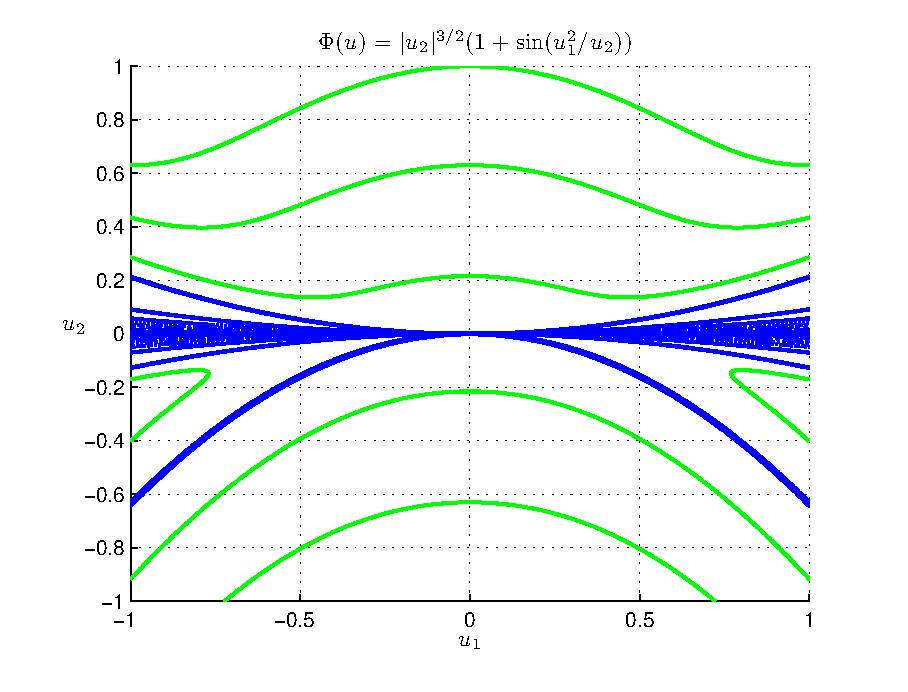
\includegraphics[width=0.7\maxpicturewidth]{your_figure.eps}
%   \center{Fig.~1. Your caption.}
% \end{figure}

\begin{references_eng}
  % Insert your list of references here. The order of items in the list must
  % agree with the order of their appearance in the text of your thesis. Use the
  % '\url' command for citing url-s: e.g., \url{http://http://www.mathopt.org/}.

\item % Reference No. 1
  Domansky~V. Repeated games with asymmetric information and random price
  fluctuations at finance markets // International Journal of Game Theory. 2007.
  V.~36, \No~2. P.~241--257.

\item Aumann R.J., Maschler M.B. Repeated Games with Incomplete Information.
  Cambridge, Massachusetts: The MIT Press, 1995.

\item % Reference No. 2
  Domansky~V.C., Kreps~V.L. Game Theoretic Bidding Model: Strategic Aspects of
  Price Formation at Stock Markets // The Journal of the New Economic
  Association. 2011. V.~11. P.~39--62.

\item Chatterjee~K., Samuelson W. Bargaining under incomplete information //
  Operations Research. 1983. V.~31, \No 5. P.~835--851.

\item P'yanykh~A.I. A Multistage Exchange Trading Model with Asymmetric
  Information and Elements of Bargaining // Moscow University Computational
  Mathematics and Cybernetics. 2016. V.~40, \No~1. P.~35--40.
  % ...

\end{references_eng}

%%%%%%%%%%%%%%%%%%%%%%%%%%%%%%%%%%%%%%%%%%%%%%%%%%%%%%%

%%% Local Variables:
%%% mode: latex
%%% TeX-master: "main"
%%% End:
